\chapter{PREESM}
\label{chapter:preesm}
In this chapter the PREESM rapid prototyping framework is introduced. First an
overview of the framework is given. Next the internal program representation in
PREESM is introduced. Last development using the PREESM framework is discussed.

\section{PREESM Overview}
\label{sec:preesmover}
The PREESM rapid prototyping framework for multicore development was used to
create a workload application for the thesis experiment described in
\ref{sec:firstexperiment}. Dataflow Models of Computation (MoC), discussed in
section \ref{sec:dataflow}, are used in PREESM to build a representation of the
application. The application is divided into parallel actors which communicate
through First In, First Out (FIFO) data queues. The actors are manually created
by the application designer in the target language. PREESM provides graphical
tools for editing the dataflow diagram and it generates a static schedule for
multicore platforms that is guaranteed to be deadlock free. PREESM combines the
generated and manually created code into a multicore executable
\cite{pelcat2014preesm}. The code generation can be configured through graphical
tools that provide hints to the schedule generation about the execution time of
different actors and rules on which cores they can be executed on. A PREESM
dataflow diagram is presented in figure \ref{preesm_example}.

\begin{figure}[h!] \label{preesm_example} \begin{center}
    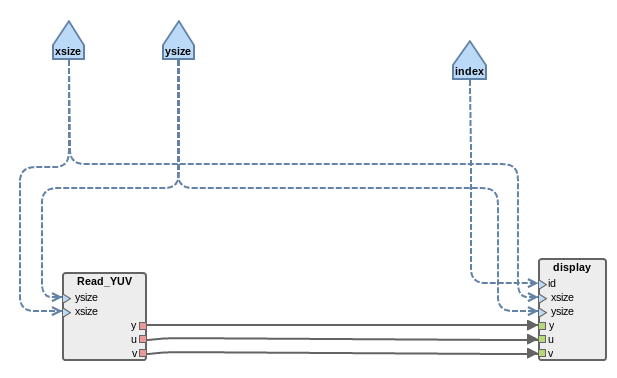
\includegraphics[width=0.99\textwidth]{images/example_preesm_diagram.png}
    \caption{A simple dataflow diagram used by PREESM} \end{center}
\end{figure}

In the experiment \ref{sec:firstexperiment} a baseline application for comparison
with OpenEM was needed. PREESM was selected because it is capable of code
generation for TMS320C6678, introduced in chapter \ref{chapter:c6678}, and its
simple and fast workflow.

\section{PREESM Internal Representations}
\label{sec:dataflow}
PREESM applications are created by combining inputs of two different
internal representations and manually created source code. The two internal
representations are described here: first the PREESM algorithm representation
PiSDF and second the PREESM hardware model.
\subsection{PiSDF}
The PREESM applications are defined using the Parameterized and Interfaced
Synchronous Dataflow Model of Computation (PiSDF)\cite{pelcat2014preesm}.

Dataflow Model of Computation (MoC) is a directed graph where each node
represents a function and the arcs are the only possible paths the data can
traverse in the graph. In the generic Dataflow MoC the number of tokens produced
or consumed by an actor is not known before execution. For example an actor may
have two output paths and it may choose to produce an output token conditionally
to either one (or both) of the paths. In contrast in Synchronous Data Flow MoC
each actor produces and consumes a pre-determined number of tokens.
\cite{lee1987synchronous} A more thorough explanation of Dataflow MoCs can be
found in \cite{lee2015introduction}.

\subsection{The System-Level Architecture Model (S-LAM)}

\section{Development with PREESM}
\label{sec:preesmdev}
